% Provenance (never printed): see sources/outline_sources.md (Year 3:
% sequence stratigraphy, accommodation and supply, systems tracts,
% cyclostratigraphy). Brief: sources/book5/BRIEFS.md, ch. 16. Curves from
% figdata/bachelor-3/shelf_model.py and lr04_periodogram.py. Exercise and
% problem values in the Book 5 scratch calculator calc/ch16.py. The Varden
% basin, its shelf and its core are invented.
\chapter{अनुक्रम स्तरिकी}\label{ch:b3:sequence-stratigraphy}

एक महाद्वीपीय सीमांत के भूकंपीय खंड में परावर्तक पुराने परावर्तकों पर आच्छादित होते हैं,
फिर द्रोणी की ओर फैलते हैं, फिर भूमि की ओर पीछे हटते हैं,
और यही प्रतिरूप ऊपर की ओर दोहराया जाता है। प्रत्येक संकुल दो दरों की होड़ का अभिलेख है:
एक दर जिससे अवसाद के लिए स्थान अवधसान और समुद्र के उठाव से बनता है,
और दूसरी दर जिससे नदियाँ उसे भरती हैं। अनुक्रम स्तरिकी इस होड़ को परतों की ज्यामिति से पढ़ती है,
और \omterm{def:b3:sequence-stratigraphy:cyclo}{चक्र-स्तरिकी}
उसकी घड़ी को उनकी मोटाई से पढ़ती है।

\begin{recall}
आवास-स्थान, यूस्टेसी, सापेक्ष समुद्र-तल, अवधसान और अवसादी द्रोणी
पुस्तक 3 (स्नातक वर्ष 1) में हैं, उसके डायाजेनेसिस और अवसादी द्रोणियों वाले अध्याय में।
समुद्री ट्रांसग्रेशन और रिग्रेशन तथा प्रथम-कोटि समुद्र-स्तर चक्र
पुस्तक 4 (स्नातक वर्ष 2) में हैं, उसके फ़ैनेरोज़ोइक पृथ्वी वाले अध्याय में;
मिलांकोविच प्राचल और जलवायवीय पुरस्सरण उसके कक्षीय बल और हिमयुग वाले अध्याय में;
आयु-मॉडल उसके जलवायु अभिलेखागार और प्रॉक्सी वाले अध्याय में
\omterm{def:b3:exploration-seismology:terminations}{ऑनलैप}, \omterm{def:b3:exploration-seismology:terminations}{डाउनलैप}, \omterm{def:b3:exploration-seismology:terminations}{टॉपलैप}, \omterm{def:b3:exploration-seismology:terminations}{अपरदनी कटान} और \omterm{def:b3:exploration-seismology:seismic-stratigraphy}{भूकंपीय स्तरिकी}
अध्याय~\ref{ch:b3:exploration-seismology} में हैं।
फ़ूरिए श्रेणी और फ़ूरिए रूपांतरण गणित की पुस्तकों में हैं।
\end{recall}

\section{आवास-स्थान, अवसाद आपूर्ति और तटरेखा}\label{sec:b3:sequence-stratigraphy:shoreline}

किसी द्रोणी के किसी भी बिंदु पर सापेक्ष समुद्र-तल $A = \dot E
+ \sigma$ की दर से बढ़ता है, अर्थात् यूस्टेटिक दर और अवधसान दर का योग; जब $A < 0$ हो, तो यह गिरता है।
किसी स्थान पर सापेक्ष समुद्र-तल वैश्विक समुद्र-तल से और उसके नीचे की भूमि को
चलाने वाली हर चीज़ से तय होता है: \omterm{def:b3:lithosphere-thermal-models:thermal-subsidence}{ऊष्मीय अवधसान}, अवसाद का भार और
उससे उत्पन्न आनमन, हिमचादर पिघलने के बाद भूपर्पटी का उछाल,
और प्लेट के नीचे प्रावार का धीमा धक्का।
बढ़ता हुआ सापेक्ष समुद्र-तल आवास-स्थान बनाता है;
अवसाद उसे भरता है। तटरेखा समुद्र की ओर खिसकती है या भूमि की ओर,
यह दोनों पर निर्भर करता है, केवल समुद्र-तल पर नहीं।
% ledger: miller20:rsl

\begin{definition}[सामान्य और बलात् रिग्रेशन]\label{def:b3:sequence-stratigraphy:regression}
\emph{सामान्य रिग्रेशन}\index{सामान्य रिग्रेशन} वह तटरेखा का समुद्र की ओर खिसकाव है
जो सापेक्ष समुद्र-तल के बढ़ते समय होता है: अवसाद आपूर्ति तटरेखा पर बने आवास-स्थान से आगे निकल जाती है।
\emph{बलात् रिग्रेशन}\index{बलात् रिग्रेशन} वह समुद्र की ओर खिसकाव है जो सापेक्ष समुद्र-तल के गिरने से
होता है: तटरेखा आपूर्ति चाहे जितनी हो, द्रोणी की ओर धकेली जाती है,
और पीछे छूटी भूमि उद्भासित होकर
अपरदित हो जाती है।
\end{definition}

\begin{definition}[तटरेखा प्रक्षेप-पथ]\label{def:b3:sequence-stratigraphy:trajectory}
\emph{तटरेखा प्रक्षेप-पथ}\index{तटरेखा प्रक्षेप-पथ} तटरेखा का समय के साथ बदलता पथ है,
जो अवसाद के संदर्भ-तंत्र में नति-खंड पर खींचा जाता है,
ताकि वह तटरेखा का क्षैतिज खिसकाव और
नीचे की परतों के सापेक्ष उसका उठना या गिरना, दोनों दिखाए।
\end{definition}

एक सरल परिच्छेद होड़ को सटीक बना देता है। तटरेखा के पीछे एक समतल शीर्ष-स्तर रहता है,
जिसकी चौड़ाई $W$ है और जो समुद्र-तल पर होता है; उसके सामने $\tan\theta$ ढाल वाला
एक अग्र-ढाल द्रोणी के तल तक उतरता है, जो $D$ ऊँचाई नीचे है।
अवसाद आपूर्ति $Q$ प्रति इकाई समय, तटरेखा के प्रति मीटर पर एक आयतन है
(खंड में प्रति इकाई समय का एक क्षेत्रफल)।

\begin{proposition}[तटरेखा प्रक्षेप-पथ]\label{prop:b3:sequence-stratigraphy:trajectory}
यदि सापेक्ष समुद्र-तल बढ़ता है ($A \ge 0$) और शीर्ष-स्तर एकसमान रूप से ऊर्ध्वाधर वृद्धि करता है,
तो तटरेखा इस दर से चलती है:
\[
\frac{\mathrm dx_s}{\mathrm dt} = \frac{Q - AW}{D};
\]
जब $Q > AW$ हो तो यह समुद्र की ओर बढ़ती है और जब $AW > Q$ हो तो पीछे हटती है। यदि सापेक्ष समुद्र-तल
गिरता है ($A < 0$), तो शीर्ष-स्तर को कुछ नहीं मिलता, और तटरेखा की गति इस प्रकार है:
\[
\frac{\mathrm dx_s}{\mathrm dt} = \frac{Q}{D} + \frac{|A|}{\tan\theta}.
\]
दोनों स्थितियों में प्रक्षेप-पथ उस कोण पर चढ़ता या उतरता है, जिसकी स्पर्शरेखा
$A/(\mathrm dx_s/\mathrm dt)$।
\end{proposition}

\begin{proof}
समय $\mathrm dt$ में शीर्ष-स्तर को समुद्र-तल पर बने रहने के लिए $AW\,\mathrm dt$ अवसाद चाहिए।
जो शेष रहता है, $(Q - AW)\,\mathrm dt$, वह अग्र-ढाल पर बिछता है,
जो $D$ ऊँचाई की दीवार है और $(Q - AW)\,\mathrm dt/D$ आगे बढ़ती है;
ऋणात्मक शेष का अर्थ है कि समुद्र शीर्ष-स्तर को उसके भरने से तेज़ी से डुबो देता है।
जब समुद्र गिरता है, तो शीर्ष-स्तर पानी के ऊपर होता है और कुछ नहीं पाता, और तटरेखा
बिना किसी अवसाद के पुराने अग्र-ढाल पर $|A|\,\mathrm dt/\tan\theta$ नीचे खिसकती है,
जबकि पूरी आपूर्ति अग्र-ढाल को $Q\,\mathrm
dt/D$ आगे बनाती है। नीचे की परतों के सापेक्ष तटरेखा $A\,\mathrm dt$ उठती है,
जिस दौरान वह $\mathrm dx_s$ खिसकती है, और यही कोण देता है।
\end{proof}

अतः \omterm{def:b3:sequence-stratigraphy:regression}{सामान्य रिग्रेशन} के लिए शीर्ष-स्तर पर बने आवास-स्थान से बड़ी आपूर्ति चाहिए,
और उसका प्रक्षेप-पथ चढ़ता है; \omterm{def:b3:sequence-stratigraphy:regression}{बलात् रिग्रेशन} आपूर्ति चाहे जितनी हो होता है,
और उसका प्रक्षेप-पथ उतरता है। दोनों दरों का अनुपात, जिसे प्रायः $A/S$ लिखा जाता है,
प्रतिरूप छाँटता है: शीर्ष-स्तर पर $A/S < 1$ हो तो प्रगलन, 1 के निकट हो तो निक्षेपण,
और उससे ऊपर हो तो पश्चगमन।
इसलिए वही समुद्र-तल वक्र एक अवसाद-समृद्ध तट पर रिग्रेशन
और एक अवसाद-विहीन तट पर ट्रांसग्रेशन दे सकता है।

\section{स्तर-ज्यामिति: अनुक्रम और तंत्र-पथ}\label{sec:b3:sequence-stratigraphy:sequences}

अध्याय~\ref{ch:b3:exploration-seismology} के परावर्तन-समापन इस विधि की शब्दावली हैं:
\omterm{def:b3:exploration-seismology:terminations}{ऑनलैप} और \omterm{def:b3:exploration-seismology:terminations}{डाउनलैप} किसी संकुल के आधार को,
और \omterm{def:b3:exploration-seismology:terminations}{टॉपलैप} तथा \omterm{def:b3:exploration-seismology:terminations}{अपरदनी कटान} उसके शीर्ष को चिह्नित करते हैं।
नति-खंड में पढ़ने पर ये तट-सीमांत को उन संकुलों में बाँटते हैं जो अनिक्षेपण या अपरदन की सतहों से सीमित होते हैं,
और उनमें से हर एक सापेक्ष समुद्र-तल के एक चक्र का अभिलेख है।

\begin{definition}[निक्षेपी अनुक्रम और अनुक्रम सीमा]\label{def:b3:sequence-stratigraphy:sequence}
\emph{निक्षेपी अनुक्रम}\index{निक्षेपी अनुक्रम} आनुवंशिक रूप से संबंधित स्तरों की एक श्रृंखला है,
जिसके भीतर कोई बड़ा अंतराल नहीं होता, और जिसका आधार और शीर्ष
असंगतियों से, या उन संगतियों से सीमित होता है जो द्रोणी में उनका विस्तार हैं।
उसकी सीमा-सतह \emph{अनुक्रम
सीमा}\index{अनुक्रम सीमा} है: सापेक्ष समुद्र-तल के गिरने के दौरान मग्नतट पर उद्भासन
और अपरदन से कटी असंगति, जो द्रोणी की ओर
सहसंबंधी संगति में बदल जाती है।
\end{definition}

\begin{definition}[तंत्र-पथ]\label{def:b3:sequence-stratigraphy:tract}
\emph{तंत्र-पथ}\index{तंत्र-पथ} निक्षेपी तंत्रों (नदी, तट, मग्नतट, ढलान) का वह समुच्चय है
जो सापेक्ष समुद्र-तल चक्र के एक भाग में एक साथ सक्रिय थे,
जिसे अनुक्रम में उसकी स्थिति,
उसकी सीमा-सतहों और स्टैकिंग प्रतिरूप से पहचाना जाता है।
इसके चार भेद किए जाते हैं:
\begin{itemize}
\item \emph{पतन-चरण तंत्र-पथ}\index{पतन-चरण तंत्र-पथ},
  सापेक्ष समुद्र-तल के गिरने के दौरान \omterm{def:b3:sequence-stratigraphy:regression}{बलात् रिग्रेशन} से निर्मित,
  पुराने मग्नतट से अलग हुए नीचे उतरते फ़ोरसेट्स:
\item \emph{निम्न-स्तर तंत्र-पथ}\index{निम्न-स्तर तंत्र-पथ},
  सापेक्ष समुद्र-तल फिर से चढ़ने लगने पर \omterm{def:b3:sequence-stratigraphy:regression}{सामान्य रिग्रेशन} से निर्मित,
  सबसे निचली तटरेखा स्थिति पर: एक पच्चर जो ऊपर की ओर जमता और आगे बढ़ता है।
\item \emph{ट्रांसग्रेसिव तंत्र-पथ}\index{ट्रांसग्रेसिव तंत्र-पथ},
  तटरेखा के भू-भाग की ओर पीछे हटने के दौरान निर्मित: पीछे हटती इकाइयाँ
  जो पुराने मग्नतट पर \omterm{def:b3:exploration-seismology:terminations}{ऑनलैप} करती हैं;
\item \emph{उच्च-स्तर तंत्र-पथ}\index{उच्च-स्तर तंत्र-पथ},
  समुद्र-तल के सापेक्षिक उठाव के उत्तरार्ध में \omterm{def:b3:sequence-stratigraphy:regression}{सामान्य रिग्रेशन} से निर्मित, जब आपूर्ति फिर से
  आवास-स्थान से आगे निकल जाती है: फ़ोरसेट्स जो आगे बढ़ते हैं और नीचे के निक्षेपों पर \omterm{def:b3:exploration-seismology:terminations}{डाउनलैप} करते हैं।
\end{itemize}
\end{definition}

\begin{definition}[ट्रांसग्रेसिव और अधिकतम प्लावन सतहें]\label{def:b3:sequence-stratigraphy:surfaces}
\emph{ट्रांसग्रेसिव सतह}\index{ट्रांसग्रेसिव सतह} निम्न-स्तर निक्षेपों के ऊपर की पहली
महत्वपूर्ण \omterm{def:b3:sequence-stratigraphy:parasequence}{प्लावन सतह} है: यह तटरेखा के रिग्रेशन से ट्रांसग्रेशन में मुड़ने को चिह्नित करती है।
\emph{अधिकतम प्लावन
सतह}\index{अधिकतम प्लावन सतह} तटरेखा की सबसे भू-भागीय स्थिति को चिह्नित करती है,
यानी ट्रांसग्रेशन से उच्च-स्तर रिग्रेशन की ओर का मोड़; उच्च-स्तर
के फ़ोरसेट्स उस पर \omterm{def:b3:exploration-seismology:terminations}{डाउनलैप} करते हैं।
\end{definition}

\begin{definition}[संघनित काट और कटी हुई घाटी]\label{def:b3:sequence-stratigraphy:condensed}
\emph{संघनित काट}\index{संघनित काट} एक पतला अंतराल है, जो तटरेखा से दूर बहुत धीरे
निक्षेपित होता है, जब समुद्र मग्नतट को जलमग्न करता है और अवसाद तट के समीप
फँस जाता है: कुछ सेंटीमीटर या डेसीमीटर
मिट्टी, जीवाश्म, ग्लॉकोनाइट या फ़ॉस्फ़ेट, जो लंबे समय का अभिलेख हो सकते हैं।
\emph{कटी हुई घाटी}\index{कटी हुई घाटी} एक नदी-घाटी है जो उजागर मग्नतट में
काटी जाती है जब सापेक्ष समुद्र-तल गिरता है, और अगले
निम्न-स्तर और ट्रांसग्रेशन के दौरान भर जाती है।
\end{definition}

\begin{omfigure}
\begin{tikzpicture}[font=\scriptsize, x=0.9cm, y=1.25cm, >=Stealth]
% older highstand deposits below the sequence boundary
\fill[black!10] (0,0) -- (14,0) -- (14,0.4) -- (10,0.6) -- (6,2.8) -- (0,3.0) -- cycle;
\draw[black!35] (1.5,2.0) .. controls (3.2,1.95) and (4.5,1.2) .. (8.5,0.45);
\draw[black!35] (3.5,2.93) .. controls (4.8,2.85) and (6,1.6) .. (10.5,0.42);
% falling-stage systems tract
\fill[red!25] (6.0,2.8) -- (7.4,2.25) -- (8.4,1.85) -- (9.4,1.35) -- (10.4,0.75) -- (10.6,0.58) -- (10,0.6) -- cycle;
\draw[red!60!black] (6.6,2.56) .. controls (7.0,2.4) and (7.5,1.95) .. (8.0,1.70);
\draw[red!60!black] (7.6,2.17) .. controls (8.0,2.0) and (8.5,1.45) .. (9.0,1.15);
\draw[red!60!black] (8.6,1.75) .. controls (9.0,1.55) and (9.5,0.9) .. (10.0,0.6);
% lowstand wedge
\fill[orange!40] (9.2,1.45) -- (10.4,1.5) -- (11.5,1.0) -- (12.6,0.6) -- (13.4,0.44) -- (10.6,0.58) -- (10.4,0.75) -- cycle;
% incised valley and its fill
\fill[orange!30] (2.9,2.9) .. controls (3.3,2.3) and (3.9,2.3) .. (4.3,2.86) -- cycle;
% transgressive systems tract
\fill[green!45!black!35] (11.5,1.0) -- (10.4,1.5) -- (9.2,1.45) -- (8.4,1.85) -- (7.4,2.25) -- (6.0,2.8) -- (1.0,2.97) -- (1.0,3.05) -- (6.0,2.95) -- (7.6,2.5) -- (9.4,1.75) -- (10.8,1.45) -- cycle;
% highstand systems tract
\fill[blue!22] (0,3.62) -- (7.5,3.42) -- (9.8,2.2) -- (11.2,1.22) -- (10.8,1.45) -- (9.4,1.75) -- (7.6,2.5) -- (6.0,2.95) -- (1.0,3.05) -- (0,3.07) -- cycle;
\draw[blue!60!black] (4.0,3.52) .. controls (5.0,3.45) and (5.8,3.1) .. (6.6,2.79);
\draw[blue!60!black] (5.6,3.47) .. controls (6.6,3.4) and (7.4,2.8) .. (8.2,2.26);
\draw[blue!60!black] (6.8,3.44) .. controls (7.8,3.35) and (8.8,2.4) .. (9.7,1.69);
% surfaces
\draw[red!70!black, very thick] (0,3.0) -- (2.9,2.9) .. controls (3.3,2.3) and (3.9,2.3) .. (4.3,2.86) -- (6.0,2.8) -- (7.4,2.25) -- (8.4,1.85) -- (9.2,1.45);
\draw[red!70!black, very thick, densely dashed] (9.2,1.45) -- (9.4,1.35) -- (10.4,0.75) -- (10.6,0.58) -- (14,0.4);
\draw[green!40!black, thick] (11.5,1.0) -- (10.4,1.5) -- (9.2,1.45);
\draw[blue!60!black, thick] (0,3.07) -- (1.0,3.05) -- (6.0,2.95) -- (7.6,2.5) -- (9.4,1.75) -- (10.8,1.45) -- (11.5,1.03) -- (12.6,0.63) -- (13.4,0.47) -- (14,0.43);
% labels
\node[blue!50!black] at (2.6,3.36) {उच्च-स्तर (HST)};
\node[green!35!black, anchor=south] at (4.8,3.92) {ट्रांसग्रेसिव (TST)};
\draw[green!35!black] (4.8,3.92) -- (4.4,3.01);
\node[red!60!black, anchor=west] at (10.1,2.45) {पतन-चरण (FSST)};
\draw[red!60!black] (10.1,2.45) -- (8.8,1.62);
\node[orange!60!black, anchor=west] at (12.2,1.55) {निम्न-स्तर (LST)};
\draw[orange!60!black] (12.2,1.55) -- (11.2,0.85);
\node[anchor=north, align=center] at (3.6,2.25) {कटी हुई\\ घाटी};
\node[red!70!black, anchor=north] at (1.4,2.95) {SB};
\node[red!70!black, anchor=north] at (12.0,0.38) {सहसंबंधी संगति};
\node[blue!60!black, anchor=west] at (12.7,1.1) {MFS};
\draw[blue!60!black] (12.7,1.1) -- (12.1,0.82);
\node[green!40!black, anchor=west] at (11.6,2.0) {TS};
\draw[green!40!black] (11.6,2.0) -- (10.9,1.27);
\node[blue!60!black, anchor=south] at (13.4,0.58) {संघनित};
\node[anchor=west, black!60] at (0.2,0.35) {पुराने निक्षेप};
\draw[->] (11.2,3.9) -- (12.6,3.9) node[right] {द्रोणी की ओर};
\end{tikzpicture}

\par\smallskip{\small नति-खंड में एक \omterm{def:b3:sequence-stratigraphy:sequence}{निक्षेपी अनुक्रम} की संरचना
(योजनाबद्ध, ऊर्ध्वाधर अतिरंजन बहुत अधिक)। \omterm{def:b3:sequence-stratigraphy:sequence}{अनुक्रम सीमा} (SB, लाल)
मग्नतट पर एक असंगति है, जिसमें एक \omterm{def:b3:sequence-stratigraphy:condensed}{कटी हुई घाटी} है, और द्रोणी में एक सहसंबंधी
संगति (धराशायी); यहाँ इसे पतन-चरण
निक्षेपों के ऊपर दर्शाया गया है। \omterm{def:b3:sequence-stratigraphy:surfaces}{ट्रांसग्रेसिव सतह} (TS) निम्न-स्तर पच्चर को ढकती है; \omterm{def:b3:sequence-stratigraphy:surfaces}{अधिकतम
प्लावन सतह} (MFS) पतले ट्रांसग्रेसिव पथ को ढकती है और द्रोणी की ओर
\omterm{def:b3:sequence-stratigraphy:condensed}{संघनित काट} में बदल जाती है; उच्च-स्तर फ़ोरसेट्स उस पर \omterm{def:b3:exploration-seismology:terminations}{डाउनलैप} करते हैं।}\label{fig:b3:sequence-stratigraphy:anatomy}
\end{omfigure}

द्रोणी में \omterm{def:b3:sequence-stratigraphy:sequence}{अनुक्रम सीमा} ठीक कहाँ से गुज़रती है, यह एक परिपाटी है, और लेखक
इस पर भिन्न हैं: कुछ इसे पतन-चरण निक्षेपों के आधार पर खींचते हैं, जहाँ पतन शुरू होता है;
दूसरे इसे उनके शीर्ष पर खींचते हैं, जहाँ वह समाप्त होता है, जैसा ऊपर के चित्र में है।
मग्नतट पर कोई अस्पष्टता नहीं है: सीमा उद्भासन और अपरदन की सतह है,
और उसके ऊपर के निक्षेप उस गिरावट से नए हैं।

बाहरी मग्नतट के एक स्थान पर नीचे से ऊपर की ओर पढ़ने पर एक अनुक्रम
इस चक्र का अभिलेख रखता है: उच्च-स्तर फ़ोरसेट्स, उद्भासन की एक सतह, संभवतः घाटी का भराव,
\omterm{def:b3:sequence-stratigraphy:surfaces}{ट्रांसग्रेसिव सतह}, पीछे हटते संस्तर, एक संघनित अंतराल,
\omterm{def:b3:sequence-stratigraphy:surfaces}{अधिकतम प्लावन सतह} पर, और फिर से उच्च-स्तर फ़ोरसेट्स। चक्रों का श्रेणीक्रम
उनके कारणों से तय होता है: प्रथम-कोटि चक्र के लिए महासागरों का खुलना
और बंद होना, छोटे चक्रों के लिए हिमचादर के आयतन और समुद्री पटल-प्रसार की गति
में परिवर्तन, और सभी चक्रों के लिए स्थानीय विवर्तनिकी तथा आपूर्ति
उत्तरदायी हैं।

\section{पैरा-अनुक्रम और स्टैकिंग प्रारूप}\label{sec:b3:sequence-stratigraphy:parasequences}

किसी \omterm{def:b3:sequence-stratigraphy:tract}{तंत्र-पथ} के भीतर भूवैज्ञानिक जिन सबसे छोटी इकाइयों को कगार पर
या कुएँ के लॉग पर मानचित्रित करता है, वे ऊपर की ओर उथली होती जाती इकाइयाँ हैं,
जो कुछ मीटर से कुछ दसियों मीटर मोटी होती हैं और जिनके ऊपर वह सतह होती है जहाँ गहरा जल अचानक लौट आता है।

\begin{definition}[पैरा-अनुक्रम और प्लावन सतह]\label{def:b3:sequence-stratigraphy:parasequence}
\emph{पैरा-अनुक्रम}\index{पैरा-अनुक्रम} प्लावन सतहों से सीमित, आनुवंशिक रूप से संबंधित संस्तरों का एक अपेक्षाकृत संगत
अनुक्रम है, जिसमें जल ऊपर की ओर उथला होता जाता है: तरंग-प्रधान तट पर अपतटीय पंक
ऊपर की ओर निचली और ऊपरी तटमुख-रेत तथा पुलिन में संक्रमित होता है।
एक \emph{प्लावन
सतह}\index{प्लावन सतह} वह सतह है जिसके पार गहरे-जल के संलक्षणी अचानक
उथले-जल वाले संलक्षणियों के ऊपर आ जाते हैं, और अचानक गहरे होने का प्रमाण मिलता है।
\end{definition}

एक एकल \omterm{def:b3:sequence-stratigraphy:parasequence}{पैरा-अनुक्रम} ऊपर की ओर मोटे कणों वाला होता जाता है, और उसका गामा-किरण लॉग,
जिसमें रेत कम और मृत्तिका अधिक होती है, ऊपर की ओर सँकरी होती एक कीप-आकृति बनाता है। किसी \omterm{def:b3:sequence-stratigraphy:tract}{तंत्र-पथ} के \omterm{def:b3:sequence-stratigraphy:parasequence}{पैरा-अनुक्रम}
एक-दूसरे पर किस प्रकार ढेर होते हैं, इससे तटरेखा की प्रवृत्ति का पता चलता है:
प्रत्येक \omterm{def:b3:sequence-stratigraphy:parasequence}{पैरा-अनुक्रम} पिछले की तुलना में समुद्र की ओर अधिक दूर बना हो (अग्रवर्ती),
उसके ऊपर बना हो (संचयी), या उसके स्थल की ओर बना हो (पश्चगामी)। ढेर के माध्यम से एक लॉग
ढेर के माध्यम से एक लॉग इस प्रवृत्ति को सीधे दिखाता है: प्रत्येक \omterm{def:b3:sequence-stratigraphy:parasequence}{पैरा-अनुक्रम}
नीचे वाले की तुलना में या तो मोटे और उथले, या समान, या बारीक और गहरे संलक्षणी पर समाप्त होता है।
उच्च-स्तर और \omterm{def:b3:sequence-stratigraphy:tract}{निम्न-स्तर तंत्र-पथ} अग्रवर्ती या संचयी रूप से ढेर होते हैं,
\omterm{def:b3:sequence-stratigraphy:tract}{ट्रांसग्रेसिव तंत्र-पथ} पश्चगामी रूप से ढेर होते हैं। अगला अध्याय ऐसे लॉग को
संलक्षणी-दर-संलक्षणी पढ़ता है।

\begin{omfigure}
\begin{tikzpicture}[font=\scriptsize, x=1cm, y=1cm]
% three logs: each parasequence a coarsening-upward wedge (grain size to the right)
% progradational
\begin{scope}[xshift=0cm]
\fill[yellow!45!brown!35] (0,0) -- (0.5,0) -- (1.4,1.1) -- (0,1.1) -- cycle;
\fill[yellow!45!brown!35] (0,1.1) -- (0.5,1.1) -- (1.8,2.2) -- (0,2.2) -- cycle;
\fill[yellow!45!brown!35] (0,2.2) -- (0.5,2.2) -- (2.2,3.3) -- (0,3.3) -- cycle;
\draw (0,0) -- (0.5,0) -- (1.4,1.1) -- (0.5,1.1) -- (1.8,2.2) -- (0.5,2.2) -- (2.2,3.3) -- (0,3.3) -- cycle;
\node[anchor=north, align=center] at (1.1,-0.1) {अग्रवर्ती\\ (तटरेखा समुद्र की ओर)};
\end{scope}
% aggradational
\begin{scope}[xshift=4.2cm]
\fill[yellow!45!brown!35] (0,0) -- (0.5,0) -- (1.8,1.1) -- (0,1.1) -- cycle;
\fill[yellow!45!brown!35] (0,1.1) -- (0.5,1.1) -- (1.8,2.2) -- (0,2.2) -- cycle;
\fill[yellow!45!brown!35] (0,2.2) -- (0.5,2.2) -- (1.8,3.3) -- (0,3.3) -- cycle;
\draw (0,0) -- (0.5,0) -- (1.8,1.1) -- (0.5,1.1) -- (1.8,2.2) -- (0.5,2.2) -- (1.8,3.3) -- (0,3.3) -- cycle;
\node[anchor=north, align=center] at (1.1,-0.1) {संचयी\\ (तटरेखा स्थिर)};
\end{scope}
% retrogradational
\begin{scope}[xshift=8.4cm]
\fill[yellow!45!brown!35] (0,0) -- (0.5,0) -- (2.2,1.1) -- (0,1.1) -- cycle;
\fill[yellow!45!brown!35] (0,1.1) -- (0.5,1.1) -- (1.8,2.2) -- (0,2.2) -- cycle;
\fill[yellow!45!brown!35] (0,2.2) -- (0.5,2.2) -- (1.4,3.3) -- (0,3.3) -- cycle;
\draw (0,0) -- (0.5,0) -- (2.2,1.1) -- (0.5,1.1) -- (1.8,2.2) -- (0.5,2.2) -- (1.4,3.3) -- (0,3.3) -- cycle;
\node[anchor=north, align=center] at (1.1,-0.1) {पश्चगामी\\ (तटरेखा स्थल की ओर)};
\end{scope}
% flooding surfaces
\foreach \s in {0,4.2,8.4} {
  \draw[omDef, thick] (\s-0.15,1.1) -- (\s+2.5,1.1);
  \draw[omDef, thick] (\s-0.15,2.2) -- (\s+2.5,2.2);
  \node[omDef, anchor=west] at (\s+2.5,1.1) {FS};
  \node[omDef, anchor=west] at (\s+2.5,2.2) {FS};
}
% grain-size axis
\draw[->] (0,3.6) -- (2.3,3.6) node[right] {मोटा};
\node[anchor=east] at (0,3.6) {पंक};
\end{tikzpicture}

\par\smallskip{\small तीन \omterm{def:b3:sequence-stratigraphy:parasequence}{पैरा-अनुक्रम} तीन तरह से ढेर किए गए हैं और कण-आकार लॉग के रूप में
दर्शाए गए हैं (दाईं ओर की चौड़ाई मोटे कणों का संकेत है)। प्रत्येक \omterm{def:b3:sequence-stratigraphy:parasequence}{पैरा-अनुक्रम} अपतटीय पंक से
तटमुख रेत तक ऊपर की ओर मोटा होता है और एक \omterm{def:b3:sequence-stratigraphy:parasequence}{प्लावन सतह} (FS) पर समाप्त होता है; प्रत्येक का
ऊपरी भाग नीचे वाले से मोटा होता है यदि ढेर अग्रवर्ती हो, समान यदि
वह संचयी हो, और बारीक यदि वह
पश्चगामी हो।}\label{fig:b3:sequence-stratigraphy:stacking}
\end{omfigure}

\begin{inthefield}[मरुस्थली कगार पर पैरा-अनुक्रम]
\begin{minipage}[t]{0.52\linewidth}\vspace{0pt}
पूर्वी यूटा के बुक क्लिफ़्स में ऊपरी क्रिटेशस तटरेखा-निक्षेप
दसियों किलोमीटर तक उजागर हैं। केनिलवर्थ सदस्य में, जिसे प्राइस से हैच मेसा तक कगारों के साथ-साथ अनुसरित किया गया,
भूवैज्ञानिकों ने तटीय-मैदान, तटमुख, आंतरिक मग्नतट और \omterm{def:b3:sequence-stratigraphy:condensed}{कटी हुई घाटी} के निक्षेपों का मानचित्रण किया, तथा
नौ ऊपर की ओर मोटे होते, तरंग-प्रधान से तूफ़ान-प्रधान \omterm{def:b3:sequence-stratigraphy:parasequence}{पैरा-अनुक्रम},
जिनकी मोटाई 7 से \qty{32}{m} थी। द्रोणी की ओर प्रत्येक \omterm{def:b3:sequence-stratigraphy:parasequence}{पैरा-अनुक्रम}
अधिकतम चार छोटे, ऊपर की ओर मोटे होते संस्तर-समूहों में बँट जाता है,
जिनकी मोटाई 2 से \qty{18}{m} है; कुछ तटमुख रेतें एक तीखे आधार पर टिकी हैं, जिन्हें
अध्ययन निम्न-स्तर के निक्षेप मानता है।
\end{minipage}\hfill
\begin{minipage}[t]{0.44\linewidth}\vspace{0pt}
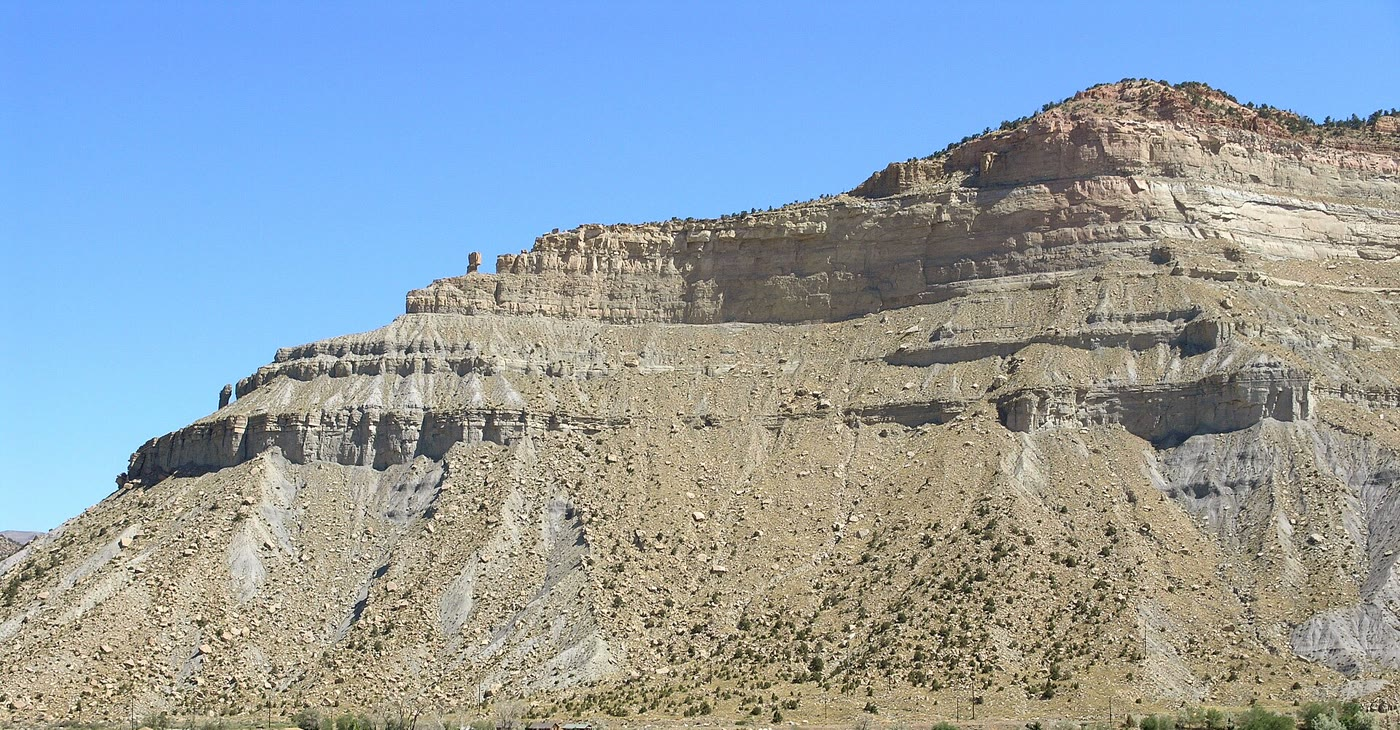
\includegraphics[width=\linewidth]{images/book5/b3-book-cliffs-helper.jpg}

{\scriptsize हेल्पर, यूटा के ऊपर के बुक क्लिफ़्स: हल्के बलुआ पत्थर की कगारें
धूसर पंकशैल ढलानों से ऊपर उभरी हैं। फ़ोटो: David Mackie, सार्वजनिक डोमेन।}
\end{minipage}
\end{inthefield}
% ledger: pattison95:kenilworth, photo:b3-book-cliffs

\section{मग्नतट का एक अग्रगामी मॉडल}\label{sec:b3:sequence-stratigraphy:model}

पिछले खंडों के नियम एक मॉडल के रूप में चलाए जा सकते हैं। वार्डन द्रोणी
एक काल्पनिक मग्नतट है: एक रैंप, जो \qty{1.5}{m/km} पर द्रोणी की ओर ढलता है और
$\sigma = 0.02 + x/1200$ \unit{m/kyr} की दर से धँसता है, वलन-मोड़ से $x$ (km) दूरी पर,
समुद्र-तल $E = -30\cos(2\pi t/400)$ (m, $t$ kyr में) के अंतर्गत, और एक नदी से पोषित,
जो तट के प्रति मीटर $Q = \qty{6000}{m^3/kyr}$ की आपूर्ति करती है। हर आधे हज़ार वर्ष के चरण पर
द्रोणी धँसती है; तब अवसाद समुद्र-तल तक एक समतल टॉपसेट भरता है,
जहाँ भी पुरानी सतह जल के नीचे हो, और उसके सामने ढाल 0.012 का एक फ़ोरसेट बनता है,
तटरेखा इस प्रकार रखी जाती है कि जोड़ा गया आयतन आपूर्ति के बराबर हो;
उजागर भूमि को कुछ नहीं मिलता और, सरलता के लिए, उसका अपरदन नहीं होता।
मॉडल निम्न-स्तर पर आरंभ होता है, स्थिर समुद्र-तल पर बने
एक पहले पच्चर के बाद।

\begin{omfigure}
\begin{tikzpicture}
\begin{groupplot}[group style={group size=1 by 2, vertical sep=0.35cm, x descriptions at=edge bottom},
  omrecord, width=0.86\linewidth, xmin=0, xmax=600,
  xtick={0,100,200,300,400,500,600},
  tick label style={font=\scriptsize}, label style={font=\small}]
\nextgroupplot[height=0.2\linewidth, ylabel={$E$ (m)}, ymin=-35, ymax=35,
  ytick={-30,0,30}]
\addplot[omDef, thick, domain=0:600, samples=121] {-30*cos(deg(2*pi*x/400))};
\nextgroupplot[height=0.3\linewidth, xlabel={समय (kyr)}, ylabel={तटरेखा $x_s$ (km)},
  ymin=0, ymax=60, ytick={0,20,40,60},
  scatter/classes={1={mark=*, red!70!black}, 2={mark=*, orange!80!black},
    3={mark=*, green!50!black}, 4={mark=*, blue!70!black}}]
% computed in figdata/bachelor-3/shelf_model.py
\addplot[scatter, only marks, mark size=0.9pt, scatter src=explicit symbolic]
  table[x=t, y=xs, meta=tract] {figdata/out/bachelor-3-shelf_model-shore.dat};
\node[font=\scriptsize, orange!60!black] at (axis cs:12,56) {LST};
\node[font=\scriptsize, green!40!black] at (axis cs:70,40) {TST};
\node[font=\scriptsize, blue!60!black] at (axis cs:160,6) {HST};
\node[font=\scriptsize, red!60!black] at (axis cs:300,22) {FSST};
\node[font=\scriptsize, orange!60!black] at (axis cs:415,57) {LST};
\node[font=\scriptsize, green!40!black] at (axis cs:520,45) {TST};
\node[font=\scriptsize, blue!60!black] at (axis cs:580,12) {HST};
\end{groupplot}
\end{tikzpicture}

\par\smallskip{\small ऊपर, वार्डन मॉडल का यूस्टेटिक समुद्र-तल;
नीचे, तटरेखा की स्थिति, \omterm{def:b3:sequence-stratigraphy:tract}{तंत्र-पथ} के अनुसार रंगीन (निम्न-स्तर
नारंगी, ट्रांसग्रेसिव हरा, उच्च-स्तर नीला, पतन-चरण लाल), केवल मॉडल के आउटपुट से
वर्गीकृत: तटरेखा पर सापेक्ष समुद्र-तल जब गिरता है तब पतन-चरण,
जब तटरेखा पीछे हटती है तब ट्रांसग्रेसिव; और निम्न-स्तर या
उच्च-स्तर जब तटरेखा बढ़ते समुद्र में आगे बढ़ती है, गिरावट के बाद या
ट्रांसग्रेशन के बाद।}\label{fig:b3:sequence-stratigraphy:series}
\end{omfigure}

ऊपर की आकृति समय के साथ तटरेखा का अनुसरण करती है, और नीचे वाली
आकृति उसके छोड़े निक्षेप दिखाती है। \omterm{def:b3:sequence-stratigraphy:tract}{तंत्र-पथ} उभरते हैं, जबकि मॉडल में
भराव और अवधसान के अलावा कोई नियम नहीं लिखा गया। आरंभ का निम्न-स्तर वेज बहुत
दूर बाहर की ओर है; बढ़ता समुद्र तटरेखा को \qty{38}{km} भूमि की ओर पहले
ट्रांसग्रेशन में धकेलता है, और समुद्र का चढ़ाव धीमा होने पर उच्च-स्तर के फ़ोरसेट्स फिर से आगे बनते हैं।
फिर पतन शुरू होता है: तटरेखा \qty{33}{km} द्रोणी की ओर धकेली जाती है
\qty{187}{kyr} में, और पतले, नीचे की ओर खिसकते फ़ोरसेट्स तथा एक उद्भासित मग्नतट
पीछे छोड़ती है; यह \omterm{def:b3:sequence-stratigraphy:tract}{पतन-चरण तंत्र-पथ} है। फिर एक नया निम्न-स्तर वेज, दूसरा
ट्रांसग्रेशन और एक नया उच्च-स्तर आते हैं। मॉडल में \omterm{def:b3:sequence-stratigraphy:regression}{बलात् रिग्रेशन} की गति
प्रतिज्ञप्ति के सूत्र से कुछ प्रतिशत के भीतर मेल खाती है; बढ़ते समुद्र के नीचे मॉडल का
टॉपसेट समान रूप से ऊपर नहीं जमता, क्योंकि अवधसान द्रोणी की ओर
बढ़ता है, और सूत्र केवल एक मार्गदर्शक है।

\begin{omfigure}
\begin{tikzpicture}
\begin{axis}[omsection, width=0.95\linewidth, height=0.42\linewidth,
  xmin=0, xmax=70, ymin=-150, ymax=40, clip=true,
  xlabel={द्रोणी की ओर दूरी (km)}, ylabel={वर्तमान ऊँचाई (m)},
  xtick={0,10,20,30,40,50,60,70}, ytick={-150,-100,-50,0},
  tick label style={font=\scriptsize}, label style={font=\small}]
% computed in figdata/bachelor-3/shelf_model.py
\addplot[fill=black!10, draw=none] table[x=x, y=z0] {figdata/out/bachelor-3-shelf_model-surfaces.dat} -- (axis cs:120,-300) -- (axis cs:0,-300) -- cycle;
\addplot[fill=orange!45, draw=none] table[x=x, y=z] {figdata/out/bachelor-3-shelf_model-poly1.dat};
\addplot[fill=green!45!black!35, draw=none] table[x=x, y=z] {figdata/out/bachelor-3-shelf_model-poly2.dat};
\addplot[fill=blue!25, draw=none] table[x=x, y=z] {figdata/out/bachelor-3-shelf_model-poly3.dat};
\addplot[fill=red!30, draw=none] table[x=x, y=z] {figdata/out/bachelor-3-shelf_model-poly4.dat};
\addplot[fill=orange!45, draw=none] table[x=x, y=z] {figdata/out/bachelor-3-shelf_model-poly5.dat};
\addplot[fill=green!45!black!35, draw=none] table[x=x, y=z] {figdata/out/bachelor-3-shelf_model-poly6.dat};
\addplot[fill=blue!25, draw=none] table[x=x, y=z] {figdata/out/bachelor-3-shelf_model-poly7.dat};
\addplot[black!45, very thin] table[x=x, y=z40] {figdata/out/bachelor-3-shelf_model-surfaces.dat};
\addplot[black!45, very thin] table[x=x, y=z80] {figdata/out/bachelor-3-shelf_model-surfaces.dat};
\addplot[black!45, very thin] table[x=x, y=z120] {figdata/out/bachelor-3-shelf_model-surfaces.dat};
\addplot[black!45, very thin] table[x=x, y=z160] {figdata/out/bachelor-3-shelf_model-surfaces.dat};
\addplot[black!45, very thin] table[x=x, y=z240] {figdata/out/bachelor-3-shelf_model-surfaces.dat};
\addplot[black!45, very thin] table[x=x, y=z280] {figdata/out/bachelor-3-shelf_model-surfaces.dat};
\addplot[black!45, very thin] table[x=x, y=z320] {figdata/out/bachelor-3-shelf_model-surfaces.dat};
\addplot[black!45, very thin] table[x=x, y=z360] {figdata/out/bachelor-3-shelf_model-surfaces.dat};
\addplot[black!45, very thin] table[x=x, y=z440] {figdata/out/bachelor-3-shelf_model-surfaces.dat};
\addplot[black!45, very thin] table[x=x, y=z480] {figdata/out/bachelor-3-shelf_model-surfaces.dat};
\addplot[black!45, very thin] table[x=x, y=z520] {figdata/out/bachelor-3-shelf_model-surfaces.dat};
\addplot[black!45, very thin] table[x=x, y=z560] {figdata/out/bachelor-3-shelf_model-surfaces.dat};
\addplot[black, thin] table[x=x, y=z600] {figdata/out/bachelor-3-shelf_model-surfaces.dat};
\addplot[black, only marks, mark=*, mark size=0.5pt] table[x=xs, y=zfinal] {figdata/out/bachelor-3-shelf_model-shore.dat};
\node[font=\scriptsize, blue!50!black] at (axis cs:6,4) {HST};
\node[font=\scriptsize, green!30!black] at (axis cs:12,-22) {TST};
\node[font=\scriptsize, red!60!black] at (axis cs:35,-25) {FSST};
\node[font=\scriptsize, orange!60!black] at (axis cs:57.5,-60) {LST};
\node[font=\scriptsize, green!30!black] at (axis cs:36,2) {TST};
\node[font=\scriptsize, blue!50!black] at (axis cs:8,26) {HST};
\end{axis}
\end{tikzpicture}

\par\smallskip{\small वार्डन मग्नतट \qty{600}{kyr} के बाद, अपनी वर्तमान
स्थिति में (ऊर्ध्वाधर अतिरंजन लगभग 170 गुना)। रंग \omterm{def:b3:sequence-stratigraphy:tract}{तंत्र-पथ} के हैं:
निम्न-स्तर नारंगी, ट्रांसग्रेसिव हरा, उच्च-स्तर नीला,
पतन-चरण लाल; धूसर भाग पुराना रैंप और पहला वेज है। पतली रेखाएँ
हर \qty{40}{kyr} पर समुद्री तल हैं; काले बिंदु हर
\qty{2}{kyr} पर तटरेखा दर्शाते हैं। गणना पाठ के अग्र मॉडल से
की गई।}\label{fig:b3:sequence-stratigraphy:section}
\end{omfigure}


तटरेखा पर सापेक्ष समुद्र-तल यूस्टेटिक उच्च-स्तर के कुछ हज़ार वर्ष बाद
गिरना शुरू होता है, क्योंकि पहले अवधसान को पार करना पड़ता है,
और यह यूस्टेटिक निम्न-स्तर से कुछ हज़ार वर्ष पहले समाप्त होता है। इस प्रकार तटरेखा पर
गिरावट यूस्टेटिक चक्र के आधे से कम समय तक चलती है, और द्रोणी जितनी
तेज़ी से धँसती है, यह उतना ही और छोटा होता है।

इस प्रकार के मॉडल किसी व्याख्या की ईमानदार परख होते हैं, और उसकी सीमाएँ
भी दिखाते हैं। वही खंड अलग-अलग इतिहासों से बन सकता है: कम आपूर्ति
के साथ तेज़ गिरावट, या अधिक आपूर्ति के साथ धीमी, या समुद्र-तल के
बजाय अवधसान में परिवर्तन, क्योंकि ज्यामिति केवल सापेक्ष समुद्र-तल और
आपूर्ति दर्ज करती है। 1970 और 1980 के दशकों में हाशियों से बने समुद्र-तल चक्रों के
वैश्विक चार्ट ने कई गिरावटों का समय तय किया, जिनकी ड्रिलिंग ने तब से
लेट क्रिटेशियस से मायोसीन तक के कुछ भागों में बड़े पैमाने पर पुष्टि की है, परंतु उनके
आयाम, जैसे मध्य ओलिगोसीन में \qty{160}{m} की गिरावट, बहुत
2 से 3 के गुणक से ऊँचे हैं। यूस्टेटिक आयाम अब
ऑक्सीजन समस्थानिकों और बैकस्ट्रिप्ड कुओं से लिए जाते हैं, और किसी
हाशिये के अनुक्रम पहले एक स्थानीय अभिलेख के रूप में पढ़े जाते हैं।
% ledger: miller20:epr, miller20:rsl

\section{चक्र-स्तरिकी}\label{sec:b3:sequence-stratigraphy:cyclo}

कई स्तर-श्रेणियाँ नियमित मोटाई-अंतरालों पर स्वयं को दोहराती हैं: मार्ल
और चूना-पत्थर के युग्म, पाँच युग्मों के गुच्छे, गुच्छों के बड़े समूह। यदि
यह पुनरावृत्ति मिलांकोविच प्राचलों से चलती है, तो चक्रों की मोटाई
समय में बदल जाती है।

\begin{definition}[चक्र-स्तरिकी और खगोलीय समस्वरण]\label{def:b3:sequence-stratigraphy:cyclo}
\emph{चक्र-स्तरिकी}\index{चक्र-स्तरिकी} अवसादी स्तर-श्रेणियों में नियमित चक्रों
की पहचान और माप करती है, और उन्हें आवधिक बल के अभिलेख के रूप में
व्याख्या करती है; मुख्यतः पृथ्वी की कक्षा और अक्ष के परिवर्तन।
\emph{खगोलीय समस्वरण}\index{खगोलीय समस्वरण} किसी स्तर-श्रेणी के चक्रों को
एक-एक करके परिकलित खगोलीय श्रेणी से मिलाकर उसे आयु प्रदान करता है
(उत्केंद्रता, तिर्यकता, पुरस्सरण या सूर्यातप), जो चक्रों को एक
आयु-मॉडल में बदल देती है।
\end{definition}

परिकलित आवर्तकाल सौर मंडल की गति के हल से प्राप्त होते हैं।
पृथ्वी की कक्षा की उत्केंद्रता का मुख्य पद \qty{405}{kyr} का है, और
\qty{100}{kyr} के आसपास चार पद हैं (95, 99, 124 और \qty{131}{kyr});
तिर्यकता का मुख्य पद \qty{41.0}{kyr} का है, जिसके छोटे पद 39.6 और
\qty{53.7}{kyr} पर हैं। जलवायवीय पुरस्सरण अक्ष के पुरस्सरण को
उपसौर की गति के साथ जोड़ता है, आवृत्तियों $p_0 + g_i$ पर, जहाँ $p_0 =
50.47''$ प्रति वर्ष और $g_i$ ग्रहीय कक्षाओं की आवृत्तियाँ हैं; इसके
मुख्य आवर्तकाल 23.7, 22.4, 19.1 और \qty{19.0}{kyr} हैं। \qty{405}{kyr}
पद सबसे स्थिर है, और पुराने स्तर-श्रेणियों के लिए एक मेट्रोनोम का काम करता है।
% ledger: la04:eccentricity, la04:obliquity, la04:precession

\begin{omfigure}
\begin{tikzpicture}
\begin{groupplot}[group style={group size=2 by 1, horizontal sep=0.5cm, y descriptions at=edge left},
  omrecord, width=0.52\linewidth, height=0.33\linewidth,
  xmin=0, xmax=0.06, ymin=0, ymax=1.18, clip=false,
  xtick={0,0.02,0.04,0.06}, xticklabels={0,0.02,0.04,0.06}, scaled x ticks=false,
  ytick={0,0.5,1}, title style={font=\small},
  tick label style={font=\scriptsize}, label style={font=\small},
  xlabel={आवृत्ति (चक्र प्रति kyr)}]
\nextgroupplot[title={(क) 0 से \qty{1000}{ka}}, ylabel={सापेक्ष शक्ति}]
\draw[black!40, densely dotted] (axis cs:0.01,0) -- (axis cs:0.01,1.05);
\draw[black!40, densely dotted] (axis cs:0.0244,0) -- (axis cs:0.0244,1.05);
\draw[black!40, densely dotted] (axis cs:0.0429,0) -- (axis cs:0.0429,1.05);
\draw[black!40, densely dotted] (axis cs:0.0526,0) -- (axis cs:0.0526,1.05);
\node[font=\scriptsize, anchor=south] at (axis cs:0.01,1.05) {100};
\node[font=\scriptsize, anchor=south] at (axis cs:0.0244,1.05) {41};
\node[font=\scriptsize, anchor=south] at (axis cs:0.0429,1.05) {23};
\node[font=\scriptsize, anchor=south] at (axis cs:0.0526,1.05) {19};
% computed in figdata/bachelor-3/lr04_periodogram.py
\addplot[omDef, thick] table[x=f, y=p] {figdata/out/bachelor-3-lr04_periodogram-young.dat};
\nextgroupplot[title={(ख) 1250 से \qty{2500}{ka}}]
\draw[black!40, densely dotted] (axis cs:0.01,0) -- (axis cs:0.01,1.05);
\draw[black!40, densely dotted] (axis cs:0.0244,0) -- (axis cs:0.0244,1.05);
\draw[black!40, densely dotted] (axis cs:0.0429,0) -- (axis cs:0.0429,1.05);
\draw[black!40, densely dotted] (axis cs:0.0526,0) -- (axis cs:0.0526,1.05);
\node[font=\scriptsize, anchor=south] at (axis cs:0.01,1.05) {100};
\node[font=\scriptsize, anchor=south] at (axis cs:0.0244,1.05) {41};
\node[font=\scriptsize, anchor=south] at (axis cs:0.0429,1.05) {23};
\node[font=\scriptsize, anchor=south] at (axis cs:0.0526,1.05) {19};
\addplot[omDef, thick] table[x=f, y=p] {figdata/out/bachelor-3-lr04_periodogram-old.dat};
\end{groupplot}
\end{tikzpicture}

\par\smallskip{\small \omterm{def:b3:sequence-stratigraphy:periodogram}{पीरियडोग्राम}, बेंथिक ऑक्सीजन-समस्थानिक स्टैक LR04 के
दो खिड़कियों में (प्रवृत्ति हटाकर, हैन टेपर, सबसे बड़े शिखर पर सामान्यीकृत);
बिंदीदार रेखाएँ 100, 41, 23 और \qty{19}{kyr} के आवर्तकाल दर्शाती हैं। (क) अंतिम
दस लाख वर्ष: \qty{100}{kyr} पट्टी प्रभावी है। (ख) \qty{2.5}{Ma} से
\qty{1.25}{Ma} तक: \qty{41}{kyr} की तिर्यकता प्रभावी है।}\label{fig:b3:sequence-stratigraphy:periodogram}
\end{omfigure}
% ledger: data:lr04, lr04:tuning

\begin{definition}[पीरियडोग्राम]\label{def:b3:sequence-stratigraphy:periodogram}
किसी श्रेणी $y_0, \dots, y_{N-1}$ का \emph{पीरियडोग्राम}\index{पीरियडोग्राम},
जो चरण $\Delta$ (समय या गहराई में) पर नमूनाकृत है, उसका माध्य और प्रवृत्ति हटाने
तथा एक टेपर $w_k$ से गुणा करने के बाद यह होता है:
\[
P(f_j) = \Bigl|\sum_{k=0}^{N-1} w_k y_k\, e^{-2\pi i f_j k\Delta}\Bigr|^2,
\qquad f_j = \frac{j}{N\Delta},\ j = 1, \dots, \frac N2:
\]
हर आवृत्ति $f_j$ पर श्रेणी की शक्ति, यानी उसके विविक्त फ़ूरियर रूपांतरण के
मापांक का वर्ग।
\end{definition}

इस \omterm{def:b3:sequence-stratigraphy:periodogram}{पीरियडोग्राम} से क्या देखा जा सकता है, यह दो संख्याएँ सीमित करती हैं। इसका आवृत्ति चरण, $1/(N\Delta)$,
अभिलेख की लंबाई का व्युत्क्रम, विभेदन है: जिन दो आवर्तकालों की आवृत्तियाँ इससे कम अंतर वाली हों,
उन्हें अलग नहीं किया जा सकता। इसकी उच्चतम आवृत्ति, नाइक्विस्ट आवृत्ति $1/(2\Delta)$, तब प्राप्त होती है
जब प्रति चक्र दो नमूने हों; इससे छोटा चक्र खोता नहीं,
बल्कि एक झूठे लंबे चक्र में मुड़ जाता है। टेपर, यहाँ एक हैन खिड़की है,
जो श्रेणी के सिरों को चिकना करता है, ताकि कोई प्रबल शिखर
अपनी शक्ति पूरे वर्णक्रम में रिसने न दे।


ऊपर के \omterm{def:b3:sequence-stratigraphy:periodogram}{पीरियडोग्राम} हल किए गए उदाहरण हैं। अंतिम दस लाख वर्ष में सबसे प्रबल
शिखर \qty{100}{kyr} पट्टी में आता है (\qty{91}{kyr} पर, जो
\qty{1000}{kyr} अभिलेख के आवृत्ति ग्रिड पर है, जिसके पड़ोसी 100 और \qty{83}{kyr} हैं),
तिर्यकता की शक्ति उसकी एक-तिहाई है और पुरस्सरण कुछ प्रतिशत;
\qty{2.5}{Ma} और \qty{1.25}{Ma} के बीच अभिलेख को तिर्यकता वहन करती है और
\qty{100}{kyr} पट्टी की शक्ति उसकी एक-छठी है। आँकड़ों में एक सावधानी अंतर्निहित है: LR04 समय-मापनी
स्वयं स्टैक को एक सरल हिम मॉडल से समस्वरित करके प्राप्त हुई थी,
जो \ang{65}\,N पर ग्रीष्म सूर्यातप से संचालित था, और अति-समस्वरण रोकने के लिए
संचित अवसादन दरों से बाधित था; अतः उसमें कक्षीय आवर्तकाल खोजना आंशिक रूप से चक्रीय है।
जो परीक्षण चक्रीय नहीं है, वह समस्वरण से पहले, गहराई में किया जाता है:
यदि चक्रों की मोटाइयों के अनुपात कक्षीय आवर्तकालों के अनुपातों से मेल खाते हैं,
तो बल-प्रेरण दर्शित हो जाता है,
और मोटाइयाँ अवसादन दर दे देती हैं।
% ledger: lr04:tuning, la04:obliquity

\begin{method}[चक्र-मोटाई से अवसादन दर]\label{met:b3:sequence-stratigraphy:cycles}
\begin{enumerate}
\item गहराई में श्रेणी का \omterm{def:b3:sequence-stratigraphy:periodogram}{पीरियडोग्राम} परिकलित कीजिए, जिसका विभेदन
  $1/L$ है (लंबाई $L$ वाले खंड के लिए) और नाइक्विस्ट सीमा $1/(2\Delta z)$;
\item महत्त्वपूर्ण शिखरों की तरंगदैर्घ्य सूचीबद्ध कीजिए, $\lambda = 1/f$;
\item उनके अनुपातों की तुलना कक्षीय आवर्तकालों के अनुपातों से कीजिए (405 : 100 : 41
  : 23, या औसत पुरस्सरण के लिए 21); तीन शिखरों का मेल एक प्रबल
  तर्क है, अकेला एक शिखर कोई नहीं;
\item प्रत्येक तरंगदैर्घ्य को उसके आवर्तकाल से भाग दीजिए: भागफल, जो
  मेल खाने चाहिए, अवसादन दर देते हैं।
\end{enumerate}
\end{method}

इस तरह प्राप्त अवसादन दर चक्र पर एक माध्य होती है
और स्थिर दर मानती है: खंड के भीतर दर में परिवर्तन शिखरों को खींच देता है,
और एक अंतराल चक्रों को चुपचाप हटा देता है। इसलिए लंबे अनुक्रमों को
परिकलित श्रेणी से चक्र-दर-चक्र समस्वरित किया जाता है,
पहले \qty{405}{kyr} चक्र को, और जहाँ ज्वालामुखीय संस्तर अनुमति दें वहाँ रेडियोमेट्रिक आयु से जाँचा जाता है।

\section{अभ्यास}

\begin{exercise}[$\star$]\label{exo:b3:sequence-stratigraphy:1}
किसी मग्नतट के एक बिंदु पर यूस्टेटिक समुद्र-तल \qty{0.5}{m/kyr} की दर से बढ़ता है और
द्रोणी \qty{0.1}{m/kyr} की दर से अवधसित होती है। सापेक्ष समुद्र-तल वृद्धि की दर
और \qty{20}{kyr} में बना आवास-स्थान परिकलित कीजिए। यदि समुद्र इसके बजाय
\qty{0.3}{m/kyr} की दर से गिरे, तो सापेक्ष दर क्या है?
\end{exercise}

\begin{exercise}[$\star$]\label{exo:b3:sequence-stratigraphy:2}
प्रत्येक स्थिति के लिए, वह \omterm{def:b3:sequence-stratigraphy:tract}{तंत्र-पथ} बताइए जो बन रहा है: (क) सापेक्ष समुद्र-तल
गिरता है, तटरेखा समुद्र की ओर खिसकती है; (ख) सापेक्ष समुद्र-तल बढ़ता है,
तटरेखा भूमि की ओर खिसकती है; (ग) सापेक्ष समुद्र-तल चक्र के अंत में धीरे बढ़ता है,
तटरेखा समुद्र की ओर खिसकती है और अग्र-ढलान \omterm{def:b3:sequence-stratigraphy:surfaces}{अधिकतम प्लावन सतह} पर \omterm{def:b3:exploration-seismology:terminations}{डाउनलैप} करते हैं;
(घ) सापेक्ष समुद्र-तल एक पतन के बाद अभी-अभी बढ़ना शुरू हुआ है,
और तटरेखा अब भी समुद्र की ओर खिसकती है।
\end{exercise}

\begin{exercise}[$\star$]\label{exo:b3:sequence-stratigraphy:3}
एक कुएँ का लॉग तीन \omterm{def:b3:sequence-stratigraphy:parasequence}{पैरा-अनुक्रम} दिखाता है, जिनमें से प्रत्येक ऊपर की ओर अधिक मोटे कणों की ओर जाता है। तीनों के शीर्ष
नीचे से गिनने पर बारीक रेत, मध्यम रेत और पुलिन-लैमिनेशन वाली मोटी रेत हैं।
स्टैकिंग प्रतिरूप, तटरेखा की गति और वे \omterm{def:b3:sequence-stratigraphy:tract}{तंत्र-पथ} बताइए जिनमें यह
संभवतः आता हो। इसके उल्टे क्रम का क्या अर्थ होगा?
\end{exercise}

\begin{exercise}[$\star$]\label{exo:b3:sequence-stratigraphy:4}
एक कगार में मार्ल और चूना-पत्थर के युग्म पाँच-पाँच के गुच्छों में समूहित दिखते हैं; एक
गुच्छा \qty{1.6}{m} मोटा है। कक्षीय आवर्तकालों की सहायता से युग्मों और गुच्छों की
व्याख्या कीजिए और गुच्छों से अवसादन दर परिकलित कीजिए।
\end{exercise}

\begin{exercise}[$\star\star$]\label{exo:b3:sequence-stratigraphy:5}
एक मग्नतट का टॉपसेट \qty{20}{km} चौड़ा है, फ़ोरसेट \qty{50}{m} ऊँचा है, और
तट के प्रति मीटर \qty{4000}{m^3/kyr} अवसाद आपूर्ति है; सापेक्ष समुद्र-तल
\qty{0.15}{m/kyr} की दर से बढ़ता है। तटरेखा की चाल परिकलित कीजिए। किस
दर से बढ़ने पर तटरेखा स्थिर रहेगी?
\end{exercise}

\begin{exercise}[$\star\star$]\label{exo:b3:sequence-stratigraphy:6}
इसी मग्नतट पर अब सापेक्ष समुद्र-तल \qty{0.2}{m/kyr} की दर से गिरता है; फ़ोरसेट
फ़ोरसेट ढलान 0.01 है। \omterm{def:b3:sequence-stratigraphy:regression}{बलात् रिग्रेशन} की चाल परिकलित कीजिए और
उसमें से वह भाग ज्ञात कीजिए जो अकेले गिरावट के कारण है।
\end{exercise}

\begin{exercise}[$\star\star$]\label{exo:b3:sequence-stratigraphy:7}
सापेक्ष समुद्र-तल \qty{0.4}{m/kyr} की दर से \qty{25}{km} चौड़े टॉपसेट पर बढ़ता है।
किस अवसाद आपूर्ति से नीचे तटरेखा पीछे हटती है? तट के प्रति मीटर
\qty{6000}{m^3/kyr} आपूर्ति और केवल \qty{10}{m} ऊँचे तटमुख के साथ, वह
कितनी तेज़ी से पीछे हटती है?
\end{exercise}

\begin{exercise}[$\star\star$]\label{exo:b3:sequence-stratigraphy:8}
उत्केंद्रता पद 94.9 और \qty{123.9}{kyr} के, तथा 94.9 और
\qty{98.9}{kyr} के पद, प्रत्येक युग्म को आवर्तलेख में अलग करने के लिए कितने लंबे अभिलेख की आवश्यकता होगी?
क्या \qty{600}{kyr} का अभिलेख यह कर सकता है?
\end{exercise}
% ledger: la04:eccentricity

\begin{exercise}[$\star\star$]\label{exo:b3:sequence-stratigraphy:9}
एक क्रोड में 20 तिर्यकता चक्र (प्रत्येक \qty{40.98}{kyr})
\qty{16.4}{m} घेरते हैं। अवसादन दर, और इसी अंतराल में दो राख-संस्तरों
के बीच का समय, जो \qty{3.1}{m} दूर हैं, परिकलित कीजिए।
\end{exercise}
% ledger: la04:obliquity

\begin{exercise}[$\star\star\star$]\label{exo:b3:sequence-stratigraphy:10}
\omterm{def:b3:sequence-stratigraphy:trajectory}{तटरेखा प्रक्षेप-पथ} का कोण परिकलित कीजिए: (क) \omterm{def:b3:sequence-stratigraphy:regression}{बलात् रिग्रेशन} में \qty{200}{m/kyr} पर,
जहाँ सापेक्ष समुद्र-तल \qty{0.4}{m/kyr} की दर से गिरता है, (ख) \omterm{def:b3:sequence-stratigraphy:regression}{सामान्य रिग्रेशन} में
\qty{50}{m/kyr} पर, जहाँ सापेक्ष समुद्र-तल \qty{0.2}{m/kyr} की दर से बढ़ता है।
एक डिग्री के भिन्नांश वाला कोण भूकंपीय खंड पर देखना आसान और
कगार पर देखना कठिन क्यों है?
\end{exercise}

\begin{exercise}[$\star\star\star$]\label{exo:b3:sequence-stratigraphy:11}
पुरस्सरण स्थिरांक $p_0 = 50.467718''$ प्रति वर्ष है और चार ग्रहीय
आवृत्तियाँ $g_5 = 4.257564$, $g_2 = 7.456665$, $g_4 = 17.910194$ और
$g_3 = 17.366595''$ प्रति वर्ष है। जलवायवीय पुरस्सरण के आवर्तकाल
$1\,296\,000''/(p_0 + g_i)$ से परिकलित कीजिए। जाँच कीजिए कि $g_2 - g_5$ और $g_4 - g_5$
405 और \qty{95}{kyr} के उत्केंद्रता पद देते हैं।
\end{exercise}
% ledger: la04:precession, la04:eccentricity

\begin{exercise}[$\star\star\star$]\label{exo:b3:sequence-stratigraphy:12}
दो द्रोणियाँ \qty{0.3}{m/kyr} की एक ही सापेक्ष समुद्र-तल वृद्धि को
\qty{100}{kyr} तक अभिलेखित करती हैं। पहली द्रोणी में यूस्टेसी \qty{0.25}{m/kyr} की दर से बढ़ती है और द्रोणी
\qty{0.05}{m/kyr} की दर से अवधसित होती है; दूसरी द्रोणी में यूस्टेसी
\qty{0.1}{m/kyr} की दर से बढ़ती है और द्रोणी \qty{0.2}{m/kyr} की दर से अवधसित होती है। दिखाइए कि दोनों
खंड एकसमान हो सकते हैं। कौन-सा अतिरिक्त प्रेक्षण दोनों
इतिहासों को अलग करता है?
\end{exercise}

\section{समस्या: वार्डन द्रोणी के समुद्र-तल}

\begin{problem}[{सप्ताहांत समस्या --- आवास-स्थान, तटरेखा प्रक्षेप-पथ
और वार्डन मग्नतट मॉडल के तंत्र-पथ, तथा एक क्रोड की घड़ी}]
\label{pb:b3:sequence-stratigraphy:1}
इस अध्याय का वार्डन मग्नतट $\sigma = 0.02 + x/1200$ की दर से अवधसित होता है
(\unit{m/kyr}, जहाँ $x$ km में है), समुद्र-तल $E = -30\cos(2\pi t/400)$ के अधीन (m,
जहाँ $t$ kyr में है), तट के प्रति मीटर \qty{6000}{m^3/kyr} अवसाद आपूर्ति और
फ़ोरसेट ढलान 0.012 के साथ। मॉडल हर \qty{50}{kyr} पर समुद्र-तल
$E$, तटरेखा की स्थिति $x_s$, तटरेखा पर सापेक्ष समुद्र-तल वृद्धि की दर $A$ और
फ़ोरसेट की ऊँचाई $D$ देता है:

\begin{center}\small
\begin{tabular}{rrrrr|rrrrr}
$t$ & $E$ & $x_s$ & $A$ & $D$ & $t$ & $E$ & $x_s$ & $A$ & $D$\\
(kyr) & (m) & (km) & (m/kyr) & (m) & (kyr) & (m) & (km) & (m/kyr) & (m)\\\hline
50 & $-21.2$ & 33.5 & 0.381 & -- & 350 & $-21.2$ & 44.6 & $-0.276$ & 25.3\\
100 & 0.0 & 15.7 & 0.504 & -- & 400 & $-30.0$ & 51.3 & 0.063 & 81.6\\
150 & 21.2 & 12.8 & 0.364 & 21.1 & 450 & $-21.2$ & 52.7 & 0.397 & 99.2\\
200 & 30.0 & 16.8 & 0.034 & 41.1 & 500 & 0.0 & 40.4 & 0.525 & --\\
250 & 21.2 & 24.0 & $-0.293$ & 45.4 & 550 & 21.2 & 22.9 & 0.372 & --\\
300 & 0.0 & 32.9 & $-0.424$ & 35.7 & 600 & 30.0 & 28.2 & 0.043 & 13.4\\
\end{tabular}
\end{center}
(डैश उस तटरेखा को दर्शाता है जो एक समतल तटीय मैदान पर पीछे हटती है, जहाँ
कोई फ़ोरसेट नहीं बनता।)

\medskip\noindent\textbf{भाग I --- आवास-स्थान।}
\begin{enumerate}
\item सबसे बड़ी यूस्टेटिक दर परिकलित कीजिए और बताइए कि वह कब होती है।
\item वलन-मोड़ पर, \qty{20}{km} और \qty{50}{km} पर अवधसान की दर परिकलित कीजिए, और
  मॉडल की सीमा, \qty{120}{km} पर भी।
\item उच्च-स्तर पर तटरेखा लगभग \qty{17.5}{km} पर है। वहाँ सापेक्ष समुद्र-तल कब
  गिरना शुरू करता है?
\item निम्न-स्तर के निकट तटरेखा लगभग \qty{50}{km} तक पहुँचती है। वहाँ सापेक्ष समुद्र-तल
  कब गिरना रुकता है?
\item यूस्टेटिक पतन के \qty{200}{kyr} की तुलना में, तटरेखा पर सापेक्ष गिरावट
  कितने समय तक चलती है? यह छोटी क्यों है?
\item \qty{30}{km} पर, एक चक्र में केवल अवधसान से कितना आवास-स्थान
  बनता है? उसकी तुलना यूस्टेटिक परास से कीजिए।
\end{enumerate}

\medskip\noindent\textbf{भाग II --- तटरेखा।}
\begin{enumerate}[resume]
\item तालिका पढ़िए: किन समयों के बीच तटरेखा समुद्र की ओर खिसकती है,
  और किन समयों के बीच भूमि की ओर?
\item एक उच्च-स्तर का टॉपसेट, जिसकी चौड़ाई \qty{15}{km} है, \qty{0.30}{m/kyr} की दर से ऊर्ध्वाधर रूप से संचित होता है,
  जिसके सामने \qty{40}{m} ऊँचा एक फ़ोरसेट है। अध्याय के प्रस्ताव से
  तटरेखा की गति परिकलित कीजिए।
\item उस टॉपसेट पर, सापेक्ष समुद्र-तल के किस उठाव की दर पर तटरेखा रुक जाएगी?
\item तालिका से \qty{300}{kyr} पर \omterm{def:b3:sequence-stratigraphy:regression}{बलात् रिग्रेशन} की गति परिकलित कीजिए।
  मॉडल \qty{204}{m/kyr} देता है: तुलना कीजिए।
\item दोनों पदों में से कौन-सा प्रबल है, आपूर्ति या पतन?
\item प्रक्षेप-पथ \qty{17.4}{km} पर \qty{16.3}{m} से उतरता है,
  (\qty{204.5}{kyr}) पर, और \qty{50.7}{km} पर \qty{-42.7}{m} तक
  (\qty{391.5}{kyr}) पर, वर्तमान ऊँचाइयों के आधार पर इसकी माध्य प्रवणता परिकलित कीजिए।
  हर बिंदु ने उसके बाद जितना अवधसान झेला है, उससे दिखाइए कि यह उतार
  \qty{59.7}{m} के यूस्टेटिक पतन के लगभग बराबर क्यों है।
\end{enumerate}

\medskip\noindent\textbf{भाग III --- तंत्र-पथ।}
\begin{enumerate}[resume]
\item तालिका से, 150 से
  \qty{600}{kyr} तक के प्रत्येक समय के लिए एक \omterm{def:b3:sequence-stratigraphy:tract}{तंत्र-पथ} निर्धारित कीजिए।
\item मॉडल पतन-चरण का आरंभ \qty{204.5}{kyr} पर रखता है
  और उसका अंत \qty{391.5}{kyr} पर; प्रश्न 3 और 4 से उनकी जाँच कीजिए।
\item इस मॉडल में \omterm{def:b3:sequence-stratigraphy:sequence}{अनुक्रम सीमा} मग्नतट पर और
  द्रोणी में कहाँ बनती है? मॉडल अपरदन नहीं करता: एक वास्तविक मग्नतट क्या दिखाएगा?
\item दूसरा ट्रांसग्रेशन \qty{559}{kyr} पर समाप्त होता है, जब तटरेखा
  \qty{18.5}{km} पर होती है। इसकी माध्य गति परिकलित कीजिए, जिसका आरंभ \qty{439.5}{kyr} पर
  \qty{52.8}{km} से हुआ था। इसके अंत पर कौन-सी सतह बनती है?
\item \omterm{def:b3:sequence-stratigraphy:tract}{ट्रांसग्रेसिव तंत्र-पथ} मग्नतट पर पतला क्यों है, और
  एक \omterm{def:b3:sequence-stratigraphy:condensed}{संघनित काट} कहाँ बनेगी?
\end{enumerate}

\medskip\noindent\textbf{भाग IV --- द्रोणी से एक क्रोड।} एक क्रोड
  जिसकी लंबाई \qty{30}{m} है और जिसे हर सेंटीमीटर पर नमूना लिया गया है, एक नियमित एकांतर दिखाता है;
  उसके गहराई-आवर्तलेख में 7.5, 2.0 और \qty{0.81}{m} तरंगदैर्घ्यों पर शिखर हैं,
  जिनमें सबसे बड़ा \qty{2.0}{m} पर है।
\begin{enumerate}[resume]
\item आवर्तलेख का आवृत्ति विभेदन और
  नाइक्विस्ट आवृत्ति परिकलित कीजिए।
\item तीनों तरंगदैर्घ्यों का सबसे बड़े शिखर से अनुपात परिकलित कीजिए, और
  उनकी तुलना कक्षीय आवर्तों से कीजिए।
\item शिखरों को आवर्त निर्धारित कीजिए और
  प्रत्येक से अवसादन दर परिकलित कीजिए। सबसे लंबा थोड़ा असहमत क्यों है?
\item क्रोड कितना समय ढकता है?
\item \qty{23.7}{kyr} के पुरस्सरण का किस तरंगदैर्घ्य पर दिखना चाहिए?
  क्या \qty{25}{cm} पर नमूना लिया गया क्रोड उसे देख सकता है, और वह कहाँ पड़ेगा?
\item तीन शिखरों का मिलान एक से अधिक मज़बूत प्रमाण क्यों है?
\item मॉडल में तटरेखा का अधिकतम द्रोणी की ओर विस्थापन बताइए,
  पतन के आरंभ से निम्न-स्तर रिग्रेशन के अंत तक।
\end{enumerate}
\end{problem}
% ledger: la04:eccentricity, la04:obliquity, la04:precession
